\documentclass[11pt]{article}
\usepackage[letterpaper, margin=1.5cm]{geometry}
\usepackage[utf8]{inputenc}
\usepackage{graphicx}
%\usepackage[uft8]{inputenc}
\usepackage{hyperref}
\usepackage{color}
\usepackage{array}
\usepackage{multirow}
\usepackage{amsmath}
\usepackage{booktabs}
\usepackage{longtable}
\usepackage{subcaption}


\newcommand{\CAVH}[1]{\begingroup\color{red}#1\endgroup}

%opening
\title{Non-protein-coding RNAs as a regulators of development in tunicates}
\author{cavh}

\begin{document}

\maketitle

%\begin{abstract}
%\end{abstract}

\section*{miRNA families origin and evolutionary perspective}
\subsection*{miRNAs in clusters}

\subsubsection*{Methods}
The starting point to detect the miRNA clusters on those species was the generation of GFF3 files with the genome coordinates of the miRNA elements. At the same time, current genome annotations from each specie was retrieved in order to determine at the same time, the position of annotated elements on those genomes. Given those elements, for each one that are not part of miRNAs annotation was designed as $\mathcal{P}_{j}$ elements, and in another way ones that are annotated as miRNAs, was identified as $\mathcal{M}_{i}$. In this way, ordered elements $\mathcal{M}_i$ and $\mathcal{M}_{i+1}$ are part of a cluster $\mathcal{C}_{k}$  $ \neg $ $\mathcal{M}_{i} \prec \mathcal{P}_{j} \prec \mathcal{M}_{i+1} $. in this way each $\mathcal{C}_{k}$ cluster was identified indepentendly and it was composed by sets of miRNA elements $M_{i}$ with a $\left\vert{P}_{k}\right\vert \ge 2$. The $M_{i}$ elements have a correspondent index $T_{i}$ that maps into the hexadecimal alphabet. Those $T_{i}$ elements could be aligned in the next steps by an implementation of a Needleman-Wunsch \cite{Needleman:70} algorithm, which have taken into account: $1:1$ matches and insertions $1:-$ or $-:1$, but not $1:1$ (mis)-matches, where the alignment program penalizes harder than a insertion. The alignment score was calculated by this score matrix:

\begin{equation}
  D_{ij} = \max \begin{cases} 
      D_{i-1,j-1}  $+ 2$ &  \textrm{Matches} \\
      D_{i-1,j-1} - ($4$) &  \textrm{(Mis)-matches} \\ 
      D_{i-1,j}   - ($1$) &  \textrm{Insertion}(a)\\
      D_{i,j-1}   - ($1$) &  \textrm{Insertion}(b)\\
      \end{cases} 
\end{equation}

In this case, all the sequences that contains at least one $M_{i}$ miRNA family represented by $T_{i}$ were collected and next, aligned in a pairwise way with all possible combinations of sequences. All the resulting alignments for each $T_{i}$ index and cleaned, taking only ones that reported alignments scores ($\mathcal{G}$) $\ge$ third quartile of the data (located in the $75$\% or greater percentage of the score distribution), creating a subset $\mathcal{B}$ with the best scored pairwise alignments.

With $\mathcal{B}$ an implementation of multiple alignments, implemented by Reztlaff (2017) was applied in order to detect the conserved blocks in all pairwise alignments. In this way the implementation allowed the detection of those conserved blocks of $M_{i} \subseteq \mathcal{B}$.

\subsubsection*{Results}
 Applying the last strategy to detect miRNA's clusters granted the option to study the conserved elements along chordate's genomes. As shown in Figure \ref{fig:sizeCluster}, directly with the location form those miRNA elements have been possible to identify the number and the length of those identified regions along all the studied genomes. In this case, the cluster that contains the greatest number of miRNAs elements ($60$) is located on \textit{D. rerio} genome: \texttt{Chromosome $4$:$28738556$-$28754891$}, for tunicates on \textit{C. intestinalis}: \texttt{Chromosome $7$:$4153284$-$4156782$} with $23$ elements, and in \textit{B. floridae}: \texttt{Bf\_V2\_118: $216744$-$220351$} only $5$ miRNAs have been detected. According to this data, complemented by the information from Figure \ref{fig:sizeCluster}, the estimation along all chordate groups shown that in cluster's detected on tunicates is possible to identify clusters that contain more miRNA's elements per Mb, in comparison to Cephalochordata and Vertebrata. %Aplicar t-student o kruskal.w para stat test.
 In complement, Table \ref{tab:detailBigClusters} describe the families miRNAs 
located inside the largest clusters fore each specie.

\begin{longtable}{p{1 cm}p{2.3 cm}p{2 cm}p{2 cm}p{2 cm}p{1.5 cm}p{1.8 cm}p{3 cm}}
\textbf{Clade}&\textbf{Specie} & \textbf{Chr} & \textbf{Start} & \textbf{End} & \textbf{Size(Mb)} & \textbf{No. miRNAs} & \textbf{Elements} \\
\toprule
C & \textit{B. floridae} & Bf\_V2\_118 & $216744$ & $220351$ & $3607$ & $5$ & bfl-mir-4869, bfl-mir-4857, bfl-mir-4862, bfl-mir-4856b, bfl-mir-4856a \\
T & \textit{O. dioica} & scaffold\_3 & $2222857$ & $2223714$ & $857$ & $6$ & odi-mir-1497e, odi-mir-1497d-2, odi-mir-1497d-1, odi-mir-1497c, odi-mir-1497b, odi-mir-1497a \\
T & \textit{B. schlosseri} & chrUn & $40003$ & $41320$ & $1317$ & $2$ & mir-233, mir-10 \\
T & \textit{C. intestinalis} & $7$ & $4153284$ & $4156782$ & $3498$ & $23$ & cin-mir-4006d, cin-mir-4006c, cin-mir-4001b-2, cin-mir-4000i, cin-mir-4006g, cin-mir-4001e, cin-mir-4001d, cin-mir-4000g, cin-mir-4006f, cin-mir-4006b, cin-mir-4001b-1, cin-mir-4000c, cin-mir-4006e, cin-mir-4000b-2, cin-mir-4001a-1, cin-mir-4000b-1, cin-mir-4002, cin-mir-4000d, cin-mir-4001h, cin-mir-4000a-2, cin-mir-4006a-2, cin-mir-4006a-3, cin-mir-4006a-1 \\
T & \textit{C. savignyi} & reftig\_16 & $3924783$ & $3925336$ & $553$ & $3$ & csa-mir-216b, csa-mir-216a, csa-mir-217 \\
T & \textit{C. savignyi} & reftig\_1 & $1335375$ & $1336487$ & $1112$ & $3$ & csa-mir-92b, csa-mir-92c, csa-mir-92a \\
V & \textit{D. rerio} & $4$ & $28738556$ & $28754891$ & $16335$ & $60$ &  \small{dre-mir-430a-18, dre-mir-430c-18, dre-mir-430b-4, dre-mir-430a-15, dre-mir-430c-18, dre-mir-430b-5, dre-mir-430a-10, dre-mir-430c-18, dre-mir-430b-5, dre-mir-430a-15, dre-mir-430c-18, dre-mir-430b-3, dre-mir-430a-10, dre-mir-430c-18, dre-mir-430b-8, dre-mir-430a-15, dre-mir-430c-18, dre-mir-430b-5, dre-mir-430a-17, miR-430, dre-mir-430b-20, dre-mir-430a-10, dre-mir-430c-18, dre-mir-430b-5, dre-mir-430i-3, dre-mir-430c-18, dre-mir-430b-3, dre-mir-430a-10, dre-mir-430c-18, dre-mir-430b-8, dre-mir-430a-11, dre-mir-430c-18, dre-mir-430b-5, dre-mir-430i-3, dre-mir-430c-18, dre-mir-430b-19, dre-mir-430a-10, dre-mir-430c-18, dre-mir-430b-5, dre-mir-430a-17, miR-430, dre-mir-430b-20, dre-mir-430a-10, dre-mir-430c-18, dre-mir-430b-5, dre-mir-430i-3, dre-mir-430c-18, dre-mir-430b-19, dre-mir-430a-10, dre-mir-430c-18, dre-mir-430b-5, dre-mir-430a-15, dre-mir-430c-18, dre-mir-430b-3, dre-mir-430a-10, dre-mir-430c-18, dre-mir-430b-8, dre-mir-430a-15, dre-mir-430c-18, dre-mir-430b-5} \\
V & \textit{L. chalumnae} & JH126646.1 & $1529355$ & $1882777$ & $353422$ & $7$ & mir-233, mir-233, mir-233, mir-598, mir-672, MIR535, mir-233 \\
\bottomrule
\caption{Details of biggest miRNA cluster for chordate species}
\label{tab:detailBigClusters}
\end{longtable}
  
\begin{figure}[ht]
\centering
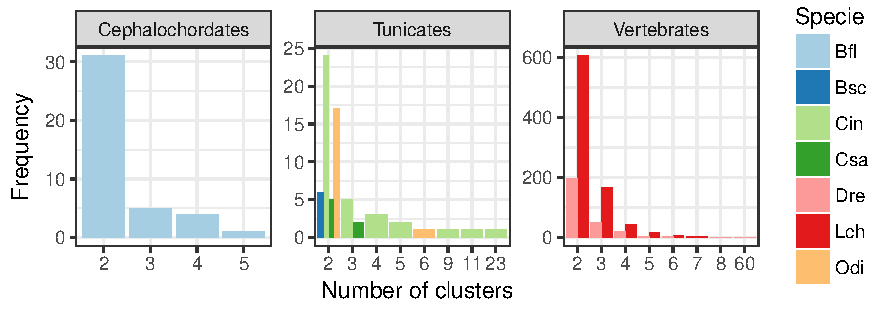
\includegraphics[scale=1]{./cluster_number.pdf} \\ 
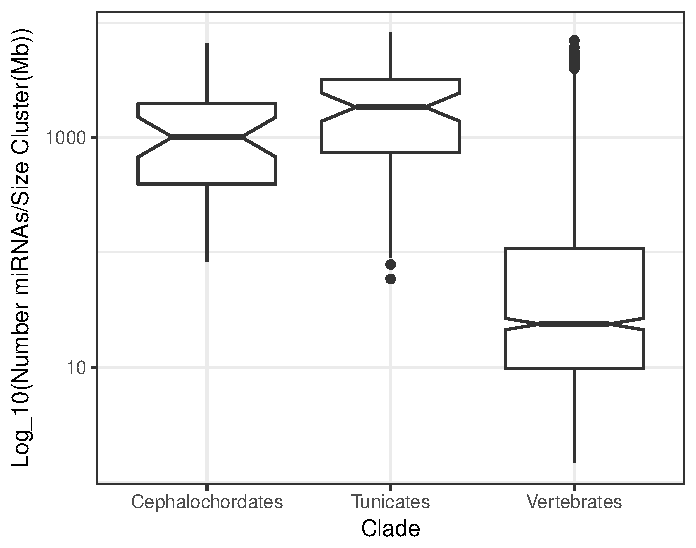
\includegraphics[scale=0.7]{./density.pdf} 
\caption{Analysis of the distribution, size and number's of cluster along chordate species.}
\label{fig:sizeCluster}
\end{figure}

Comparison between miRNA clusters have been calculated in order to access to the 
most conserved set of miRNA families inside in a cluster. Conserved blocks have 
been detected on all species and the following miRNAs are inside a 
cluster and also sharing conserved blocks with another species: let-7, mir-1, 
MIR1122, mir-130, mir-132, mir-133, mir-135, mir-146, mir-15, mir-17, mir-181, 
mir-183, MIR1846, mir-186, mir-19, mir-193, mir-216, mir-219, mir-23, mir-24, 
mir-242, mir-25, mir-27, mir-286, mir-29, mir-2985-2, mir-30, mir-34, mir-395, 
mir-454, mir-489, MIR535, mir-8, mir-9. Details about the nature of this 
elements are described on Figure \ref{fig:clusterDetail} \CAVH{Working...}.

\begin{figure}[ht!]
\centering
    \begin{subfigure}[t]{1\textwidth}
        \centering
        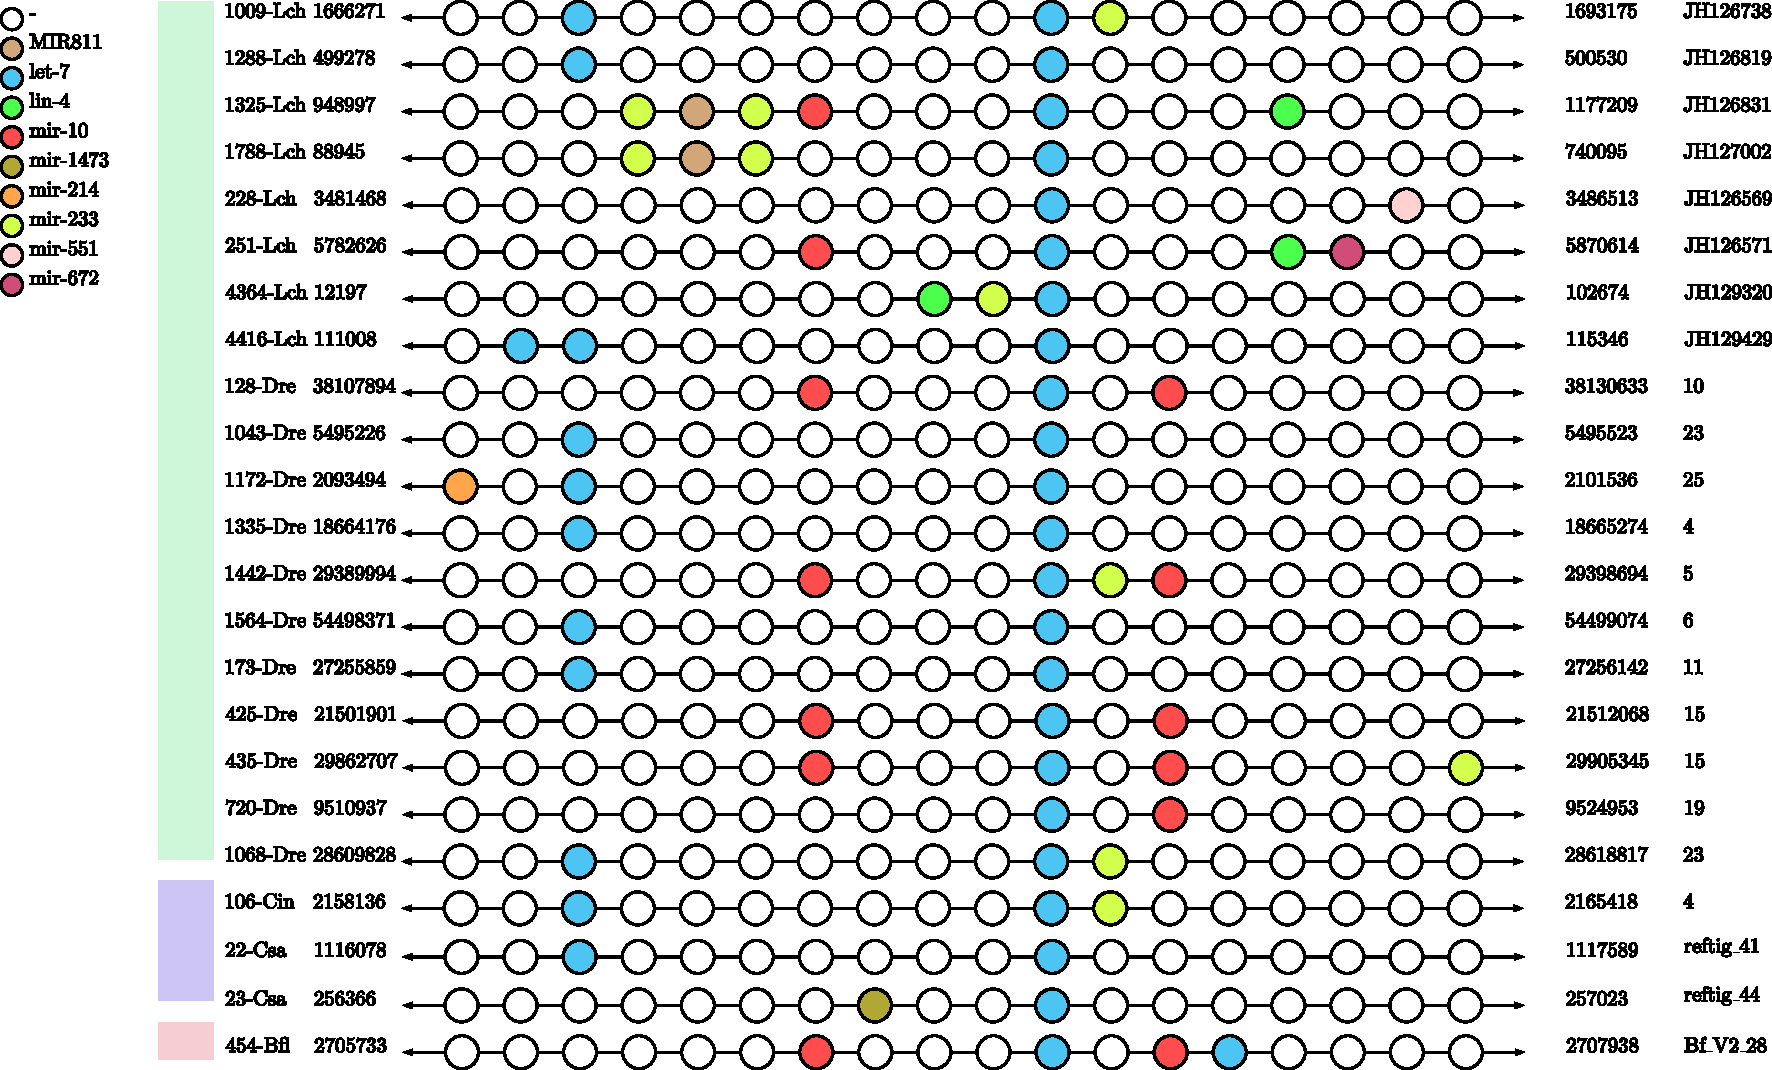
\includegraphics[height=9 cm]{Cluster_images/let-7_101_128}
        \caption{let-7}
    \end{subfigure}
    \\
    \begin{subfigure}[t]{0.45\textwidth}
        \centering
        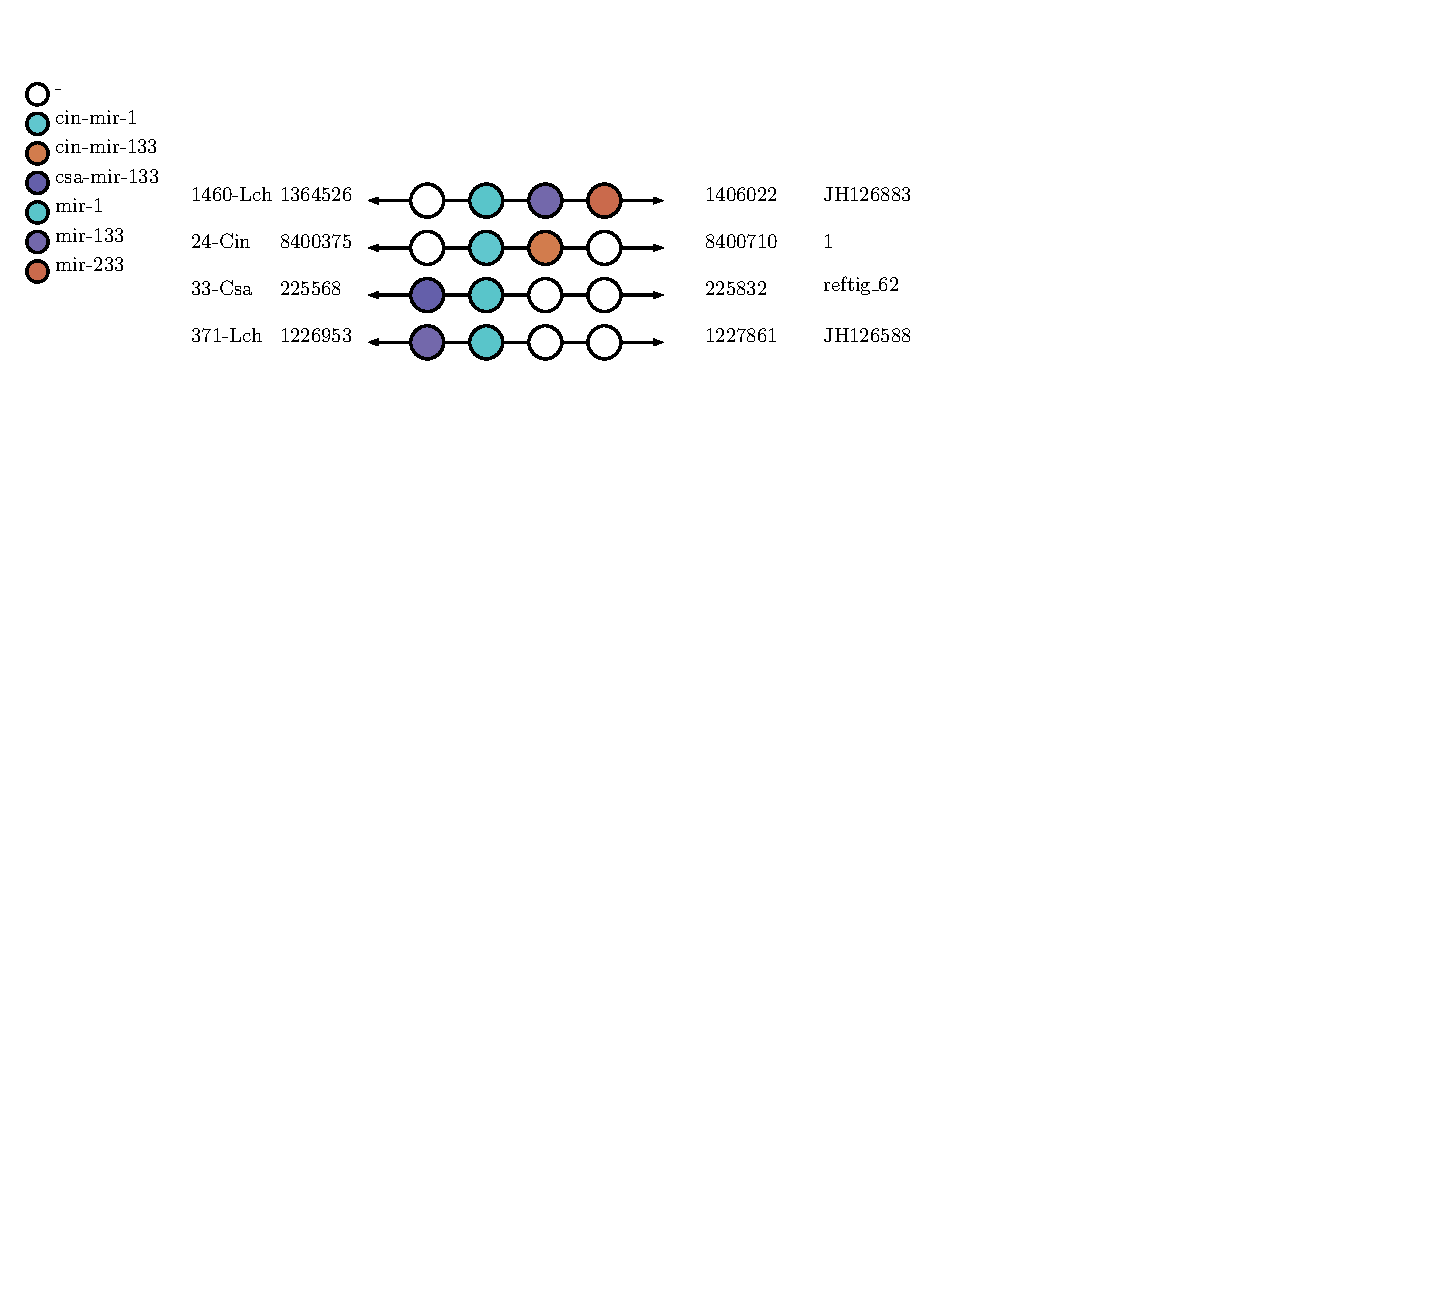
\includegraphics[height=1.2 cm]{Cluster_images/mir-1_119_33}
        \caption{mir-1/mir-133}
     \end{subfigure}
        ~
     \\
    \begin{subfigure}[t]{0.45\textwidth}
        \centering
        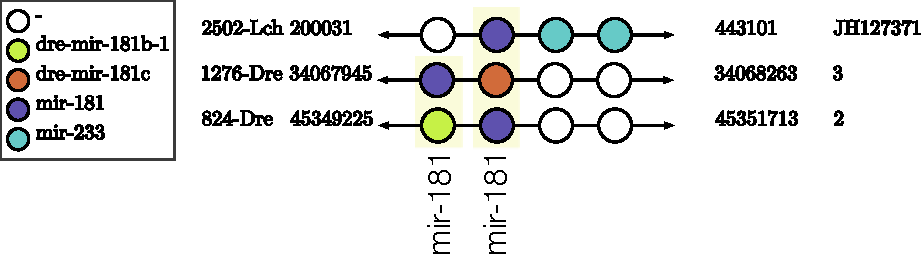
\includegraphics[height=1.2 cm]{Cluster_images/mir-181_105_2502}
        \caption{mir-181}
       \end{subfigure}
        ~
         \begin{subfigure}[t]{0.45\textwidth}
        \centering
        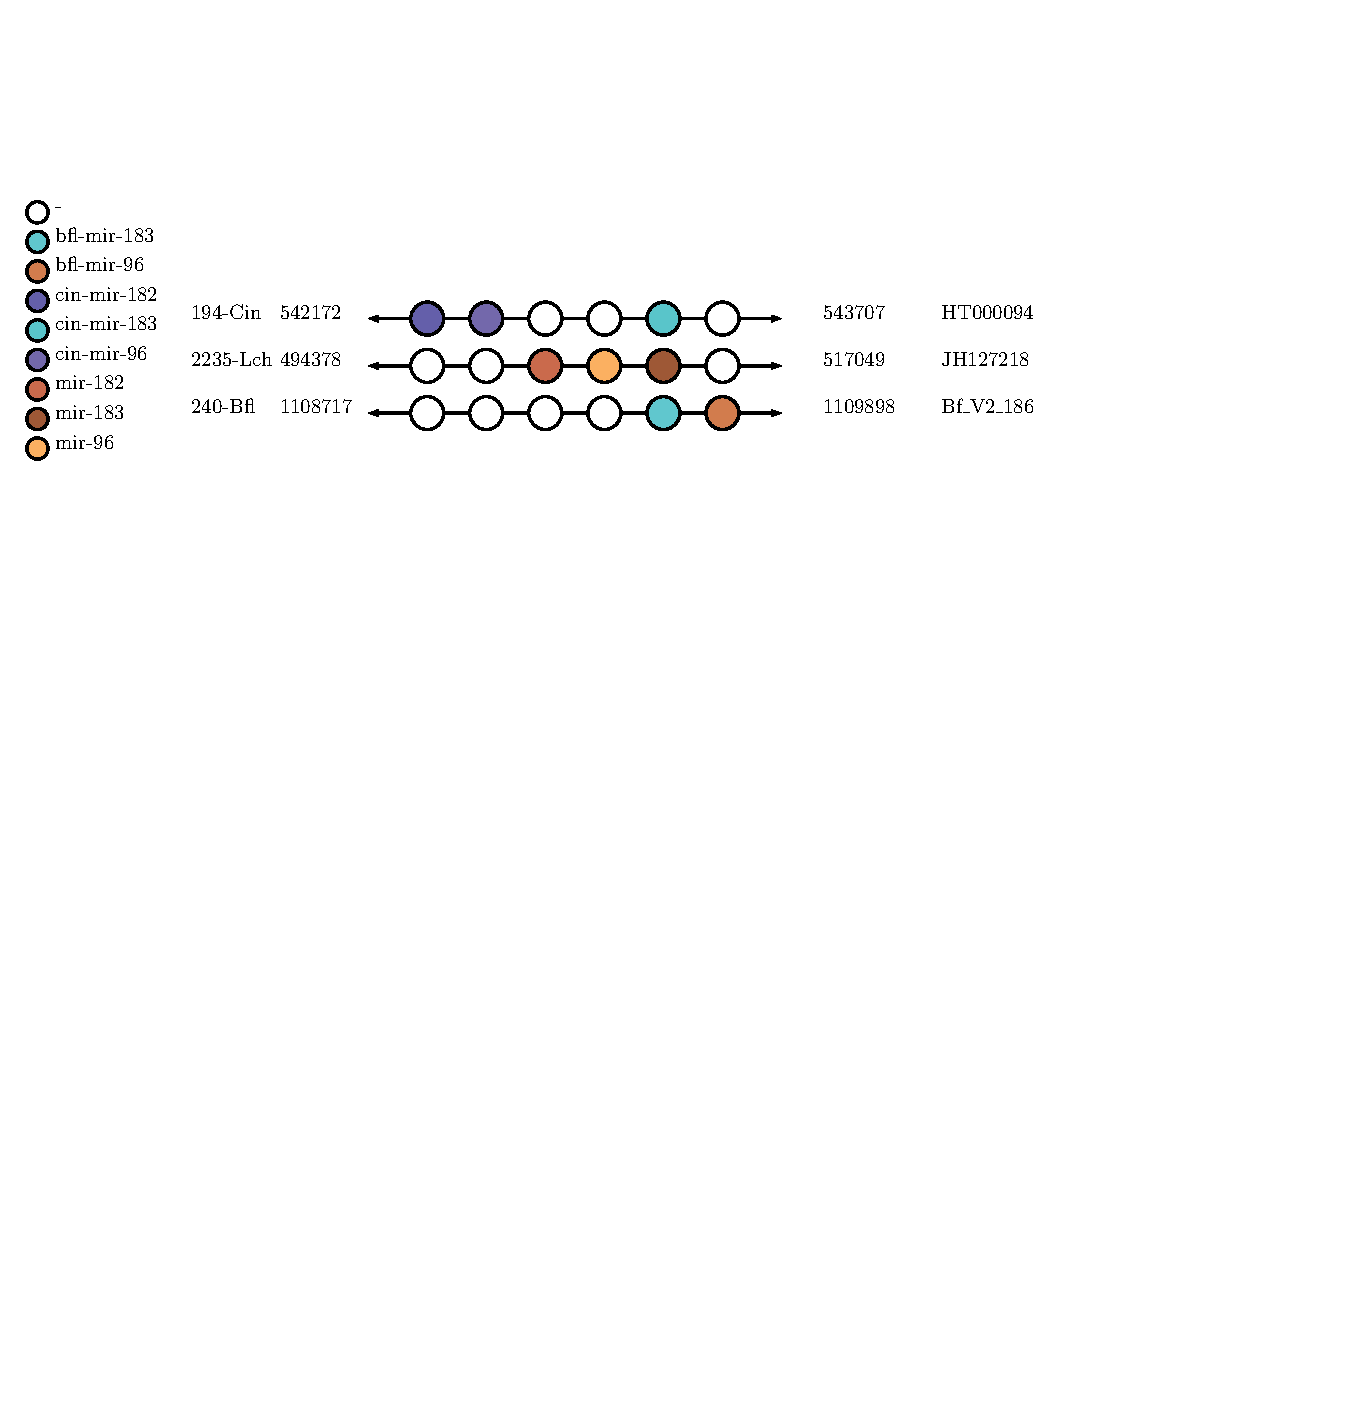
\includegraphics[height=1.2 cm]{Cluster_images/mir-183_132_240}
        \caption{mir-183}
    \end{subfigure}
    \\
    \begin{subfigure}[t]{0.45\textwidth}
        \centering
        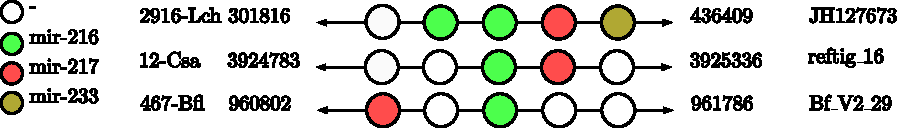
\includegraphics[height=1.2 cm]{Cluster_images/mir-216_126_467}
        \caption{mir-216/mir-217}
       \end{subfigure}
     \\
    \begin{subfigure}[t]{0.45\textwidth}
        \centering
        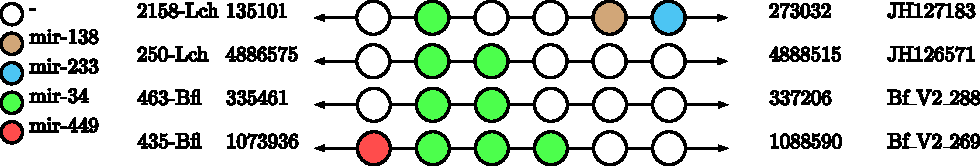
\includegraphics[height=1.2 cm]{Cluster_images/mir-34_11A_435}
        \caption{mir-34}
       \end{subfigure}
        ~
         \begin{subfigure}[t]{0.45\textwidth}
        \centering
        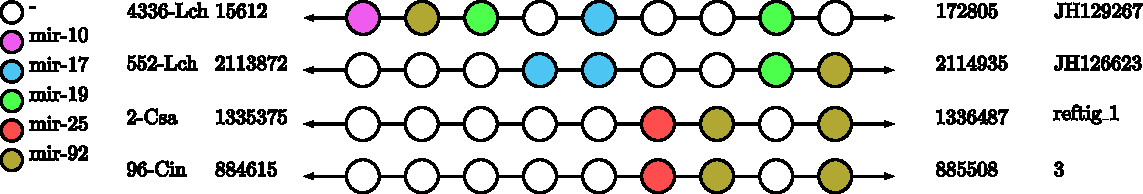
\includegraphics[height=1.2 cm]{Cluster_images/mir-92_281_4336}
        \caption{mir-92}
    \end{subfigure}
    \\
    \begin{subfigure}[t]{1\textwidth}
        \centering
        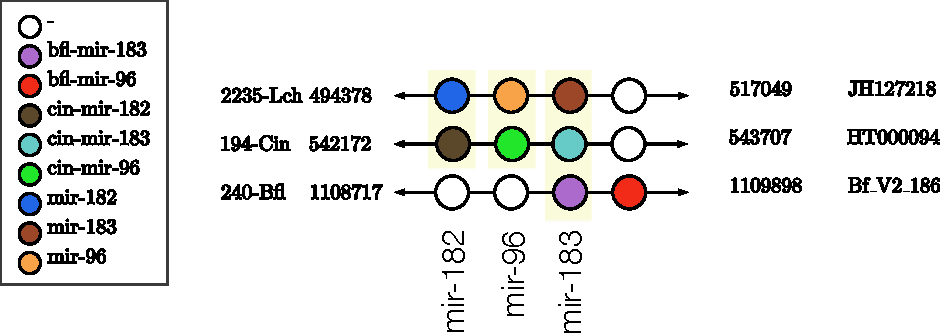
\includegraphics[height=1.2 cm]{Cluster_images/mir-96_138_240}
        \caption{mir-96}
    \end{subfigure}
    \caption{Multiple alignments of miRNA's clusters. \textbf{Prot}: Protostomata, \textbf{Brfl}: \textit{B. floridae}, 
\textbf{Oidi}: \textit{O. dioica}, \textbf{Dvex}: \textit{D. vexillum}, 
\textbf{Ciin}: \textit{C. intestinalis}, \textbf{Cisa}: \textit{C. savignyi}, 
\textbf{Ciro}: \textit{C. robusta}, \textbf{Sath}: \textit{S. thompsoni}, 
\textbf{Mata}: \textit{M. oculata}, \textbf{Mlta}: \textit{M. occulta}, 
\textbf{Mlis}: \textit{M. occidentalis}, \textbf{Bosc}: \textit{B. schlosseri}, 
\textbf{Haro}: \textit{H. roretzi}, \textbf{Pema}: \textit{P. marinus}, 
\textbf{Dare}: \textit{D. rerio}, \textbf{Lach}: \textit{L. chalumnae}, 
\textbf{Xetr}: \textit{X. tropicalis} and \textbf{Anca}: \textit{A. 
carolinensis}.}
\end{figure}

\subsection*{To complete the tree of loss and gain of families}
\subsubsection*{Methods}

The initial eight chordates genomes from chordate species: 
\textit{Branchiostoma floridae}, \textit{Botryllus schlosseri}, 
\textit{Ciona intestinalis}, \textit{Ciona savignyi}, \textit{Danio rerio}, 
\textit{Didemnum vexillum}, \textit{Latimeria chalumnae} and 
\textit{Oikopleura dioica}, were analyzed through homology searches at sequence 
level and a posterior validation by secondary structure alignments against 
pre-build metazoan-covariance models, as reported by \cite{velandia:2016}. The 
final set of miRNAs was generated on a GFF file, reporting all the genome 
coordinates from each miRNA element. Given these information, miRNA families 
names were obtained from miRBase, with the miFam.dat file, which contains the 
relationships between miRNA specific annotations for each specie and their 
correspondent miRNA family. These annotations were compared against the last 
report of miRNAs families reported by \cite{Hertel2015}. In case that the 
obtained miRNA family was not included neither miRBase or miRNAs matrix, a new 
label were designed to detect those specific elements. At the same time, from 
the reported matrix was considered the reported families from the following 
vertebrates: \textit{Anolis carolinensis}, \textit{Petromyzon marinus} and 
\textit{Xenopus tropicalis}. At the same time, two new reports of miRNAs on 
tunicates were included on this matrix from: \textit{Salpa thompsoni} 
\cite{Jue2016} and \textit{Halocynthia roretzi} \cite{Wang2017}. At now, three 
new genomes from the \textit{Molgula sp.} genus were reported \cite{Stolfi2014} 
and the genome sequences have been obtained from ANISEED 
\footnote{\url{https://www.aniseed.cnrs.fr/}} \cite{Brozovic2017}.

For the latter species, homology BLAST searches were performed. All hairpin 
sequences from miRBase (v. 21) \cite{Kozomara2014} were used as queries against 
those genomes. After that, in order to obtain the best miRNA 
candidates, mature sequences were searched on previously detected hairpin 
candidates. This strategy also include the new reported genome from 
\textit{Ciona robusta} reported on ANISEED. 

In this way, the initial miRNA matrix from \cite{Hertel2015} was updated 
with the information retrieved from detection of miRNAs families and also, with 
the inclusion from candidates in new reported genomes (\textit{H. roretzi}, 
\textit{S. thompsoni}, \textit{M. occidentalis}, \textit{M. occulta} and 
\textit{M. oculata}). Moreover, the phylogenetic distribution from Tunicate 
clade have been obtained from \cite{Simion2016}. And the final tree has been 
completed with the inclusion of one cephalochordata (\textit{B. floridae}) and 
five vertebrates (\textit{A. carolinensis}, \textit{D. rerio}, \textit{L. 
chalumnae}, \textit{P. marinus} and \textit{X. tropicalis}).

Additionally, in the final matrix only families that have presence in at least 
two species were considered, except for the miRNAs families that belongs from 
Protostomata group (Prot). This updated matrix and the phylogenetic 
distribution of the species in Newick format were the input files for Count 
program \cite{Csuos2010} in order to reconstruct the corresponding miRNAs family 
history by the implemented Dollo parsymony.

\subsection*{Results}
The updated matrix of miRNAs reported $691$ families, including the miRBase 
annotations and the homology predictions validated by secondary structure 
alignments as shown in Figure \ref{fig:matrixmirnas}. For tunicates miRNAs, the
majority have been detected/annotated in \textit{C. intestinalis} (now referred 
as \textit{C. robusta}) where exists miRBase annotations for specie-specific 
miRNAs families and also were annotated a set of miRNAs validated by secondary 
structure comparisons against metazoan-specific covariance models \CAVH{Cite 
Cristian Master Thesis}. Along this distribution of miRNAs families, $2$ 
families are conserved along all the species, even in Protostomata clade and 
vertebrates. Also, additional $8$ families complement the $10$ most conserved 
set of miRNAs that have been detected by this strategy, as follows: mir-124, 
mir-8, mir-153, mir-1, mir-216, mir-190, mir-133 and mir-31. 
From the most conserved miRNAs families \textit{O. dioica} and 
\textit{S. thompsoni} has been lost about $40$\% and $50$\% of those 
conserved families, respectively. 


At the same time, the state of those conserved elements in Protostomata, 
Cephalochordata and Vertebrata show evident lost about $\sim 10$\% of the 
families.
The general trend in Craniata shows an increment of conserved 
families, sometimes with the possibility of trace the presence from \textit{P. 
marinus} and identifying $16$ conserved candidates along all species in the 
clade that are not reported in another clades (mir-15, -181, -23, -199, 
-24, -204, -128, -221, -205, -192, -132, -138, -145, -143, -451 and 
-456). Specifically, exists $44$ miRNAs that have been identified at least 
on $2$ species of tunicates but not in Cephalochordata or 
Vertebrata \footnote{mir-368, mir-450, mir-3, mir-340, mir-335, 
mir-297,mir-466, mir-287, mir-11, mir-374, mir-664, mir-467, mir-568, mir-876, 
mir-1497, mir-281, mir-553, mir-200, mir-1473, mir-1469, mir-92\_2, mir-1502, 
mir-4079, mir-3149, mir-1277, mir-8915, mir-3533, cin-mir-4034, cin-mir-4047, 
cin-mir-4049, cin-mir-4052, cin-mir-4053, cin-mir-4054, 
cin-mir-4065, cin-mir-4072, cin-mir-4086, cin-mir-4093, 
cin-mir-4101, cin-mir-4123, cin-mir-4171, cin-mir-4220, 
cin-mir-4000c, cin-mir-4010, cin-mir-4029}, but from those candidates only $7$ 
(mir-1497, -281, -1473, -200, -92, -1502 and -4079) are previously reported as 
tunicate specific, the other ones have been reported also in vertebrates 
(mir-1277, -297, -3533, -466, -467, -568, -374, -450, -876, -8915, -3149, -355, 
-340, -553) and in insects (mir-3 and mir-11). In complement Figure 
\ref{fig:venn}, compares the shared families of miRNAs in all the studied 
chordate species. Is important to annotate that the candidates from \textit{P. 
marinus}, \textit{D. rerio}, \textit{L. chalumnae} and \textit{A. carolinensis} 
have been grouped with the Vertebrates label. In this case, in overall is 
possible to found $47$ miRNAs families that are at least in one specie in 
Vertebrata clade and is not shared with the other chordates. The homology 
searches allowed scan the annotated miRNAs families on new reported genomes 
assemblies from tunicates, as \textit{H. roretzi} and \textit{S. thompsoni}, 
including additional possible candidates to the reported set, that in case of 
\textit{H. roretzi} has been reported as experimental candidates from 
\textit{C. intestinalis} reported families. At the same time, \textit{D. 
vexillum} share a high number of elements with \textit{B. schlosseri} and 
species included on Vertabrata ($9$) and specifically with vertebrates ($13$). 
At the same time, remain a set of candidates old candidates that are shared 
between \textit{Protostomata}, \textit{B. floridae} and \textit{Vertebrata}: 
mir-193, mir-375 and mir-182. Different to the set of candidates those are 
basal in this study: \textit{Protostomata} and \textit{B. floridae}, whose 
share $2$ families: mir-71 and mir-242\_2.

\begin{figure}[htp]
\centering 
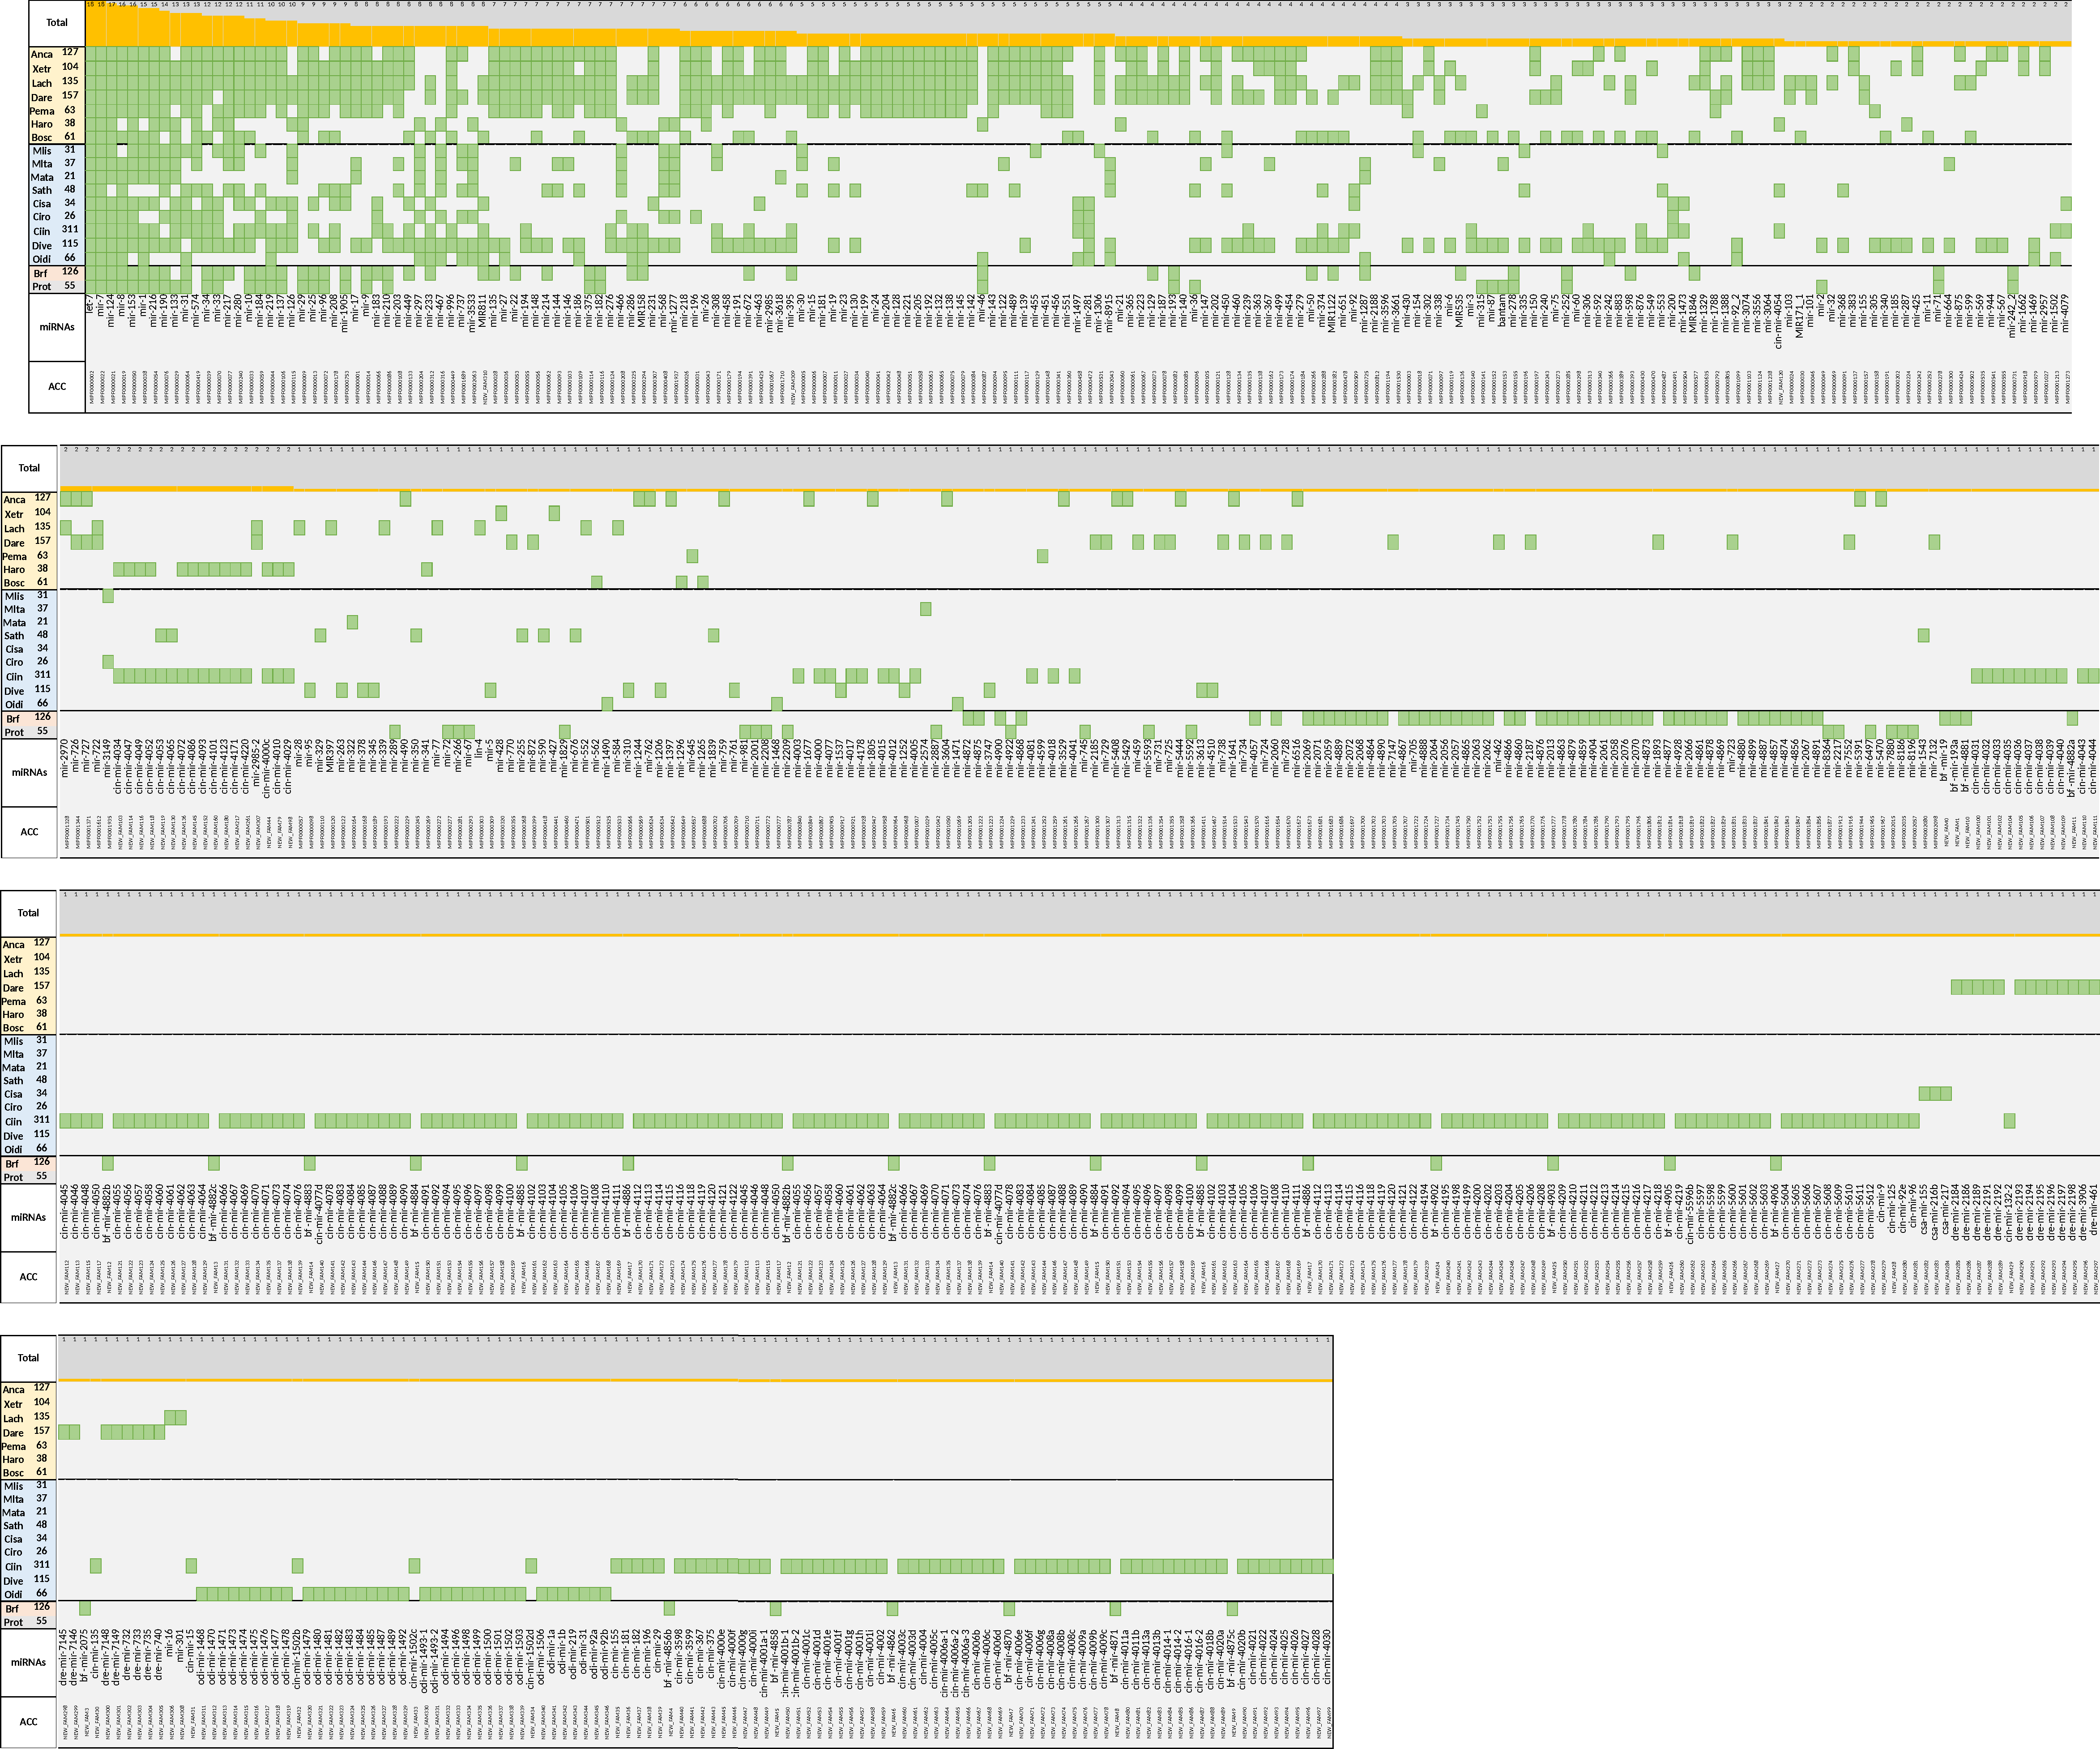
\includegraphics[draft=false,width=\textwidth]{./Images/miRNA_matrix}
\caption{Absence/Presence Matrix of miRNAs families along Bilaterian species. 
\textbf{Prot}: Protostomata, \textbf{Brfl}: \textit{B. floridae}, 
\textbf{Oidi}: \textit{O. dioica}, \textbf{Dvex}: \textit{D. vexillum}, 
\textbf{Ciin}: \textit{C. intestinalis}, \textbf{Cisa}: \textit{C. savignyi}, 
\textbf{Ciro}: \textit{C. robusta}, \textbf{Sath}: \textit{S. thompsoni}, 
\textbf{Mata}: \textit{M. oculata}, \textbf{Mlta}: \textit{M. occulta}, 
\textbf{Mlis}: \textit{M. occidentalis}, \textbf{Bosc}: \textit{B. schlosseri}, 
\textbf{Haro}: \textit{H. roretzi}, \textbf{Pema}: \textit{P. marinus}, 
\textbf{Dare}: \textit{D. rerio}, \textbf{Lach}: \textit{L. chalumnae}, 
\textbf{Xetr}: \textit{X. tropicalis} and \textbf{Anca}: \textit{A. 
carolinensis}. }
\label{fig:matrimirnas}
\end{figure}

\begin{figure}[ht!]
\centering
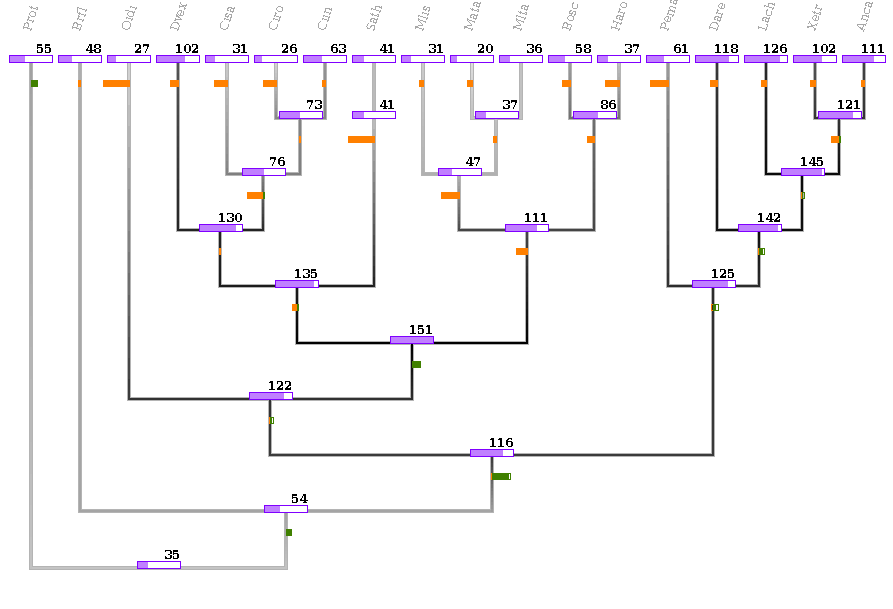
\includegraphics[width=\textwidth]{./Images/last_tree.png}
\caption{Dollo parsymony of miRNAs families distribution in some 
chordates genomes}.
\label{fig:dollotree}
\end{figure}

\begin{figure}[ht!]
\centering
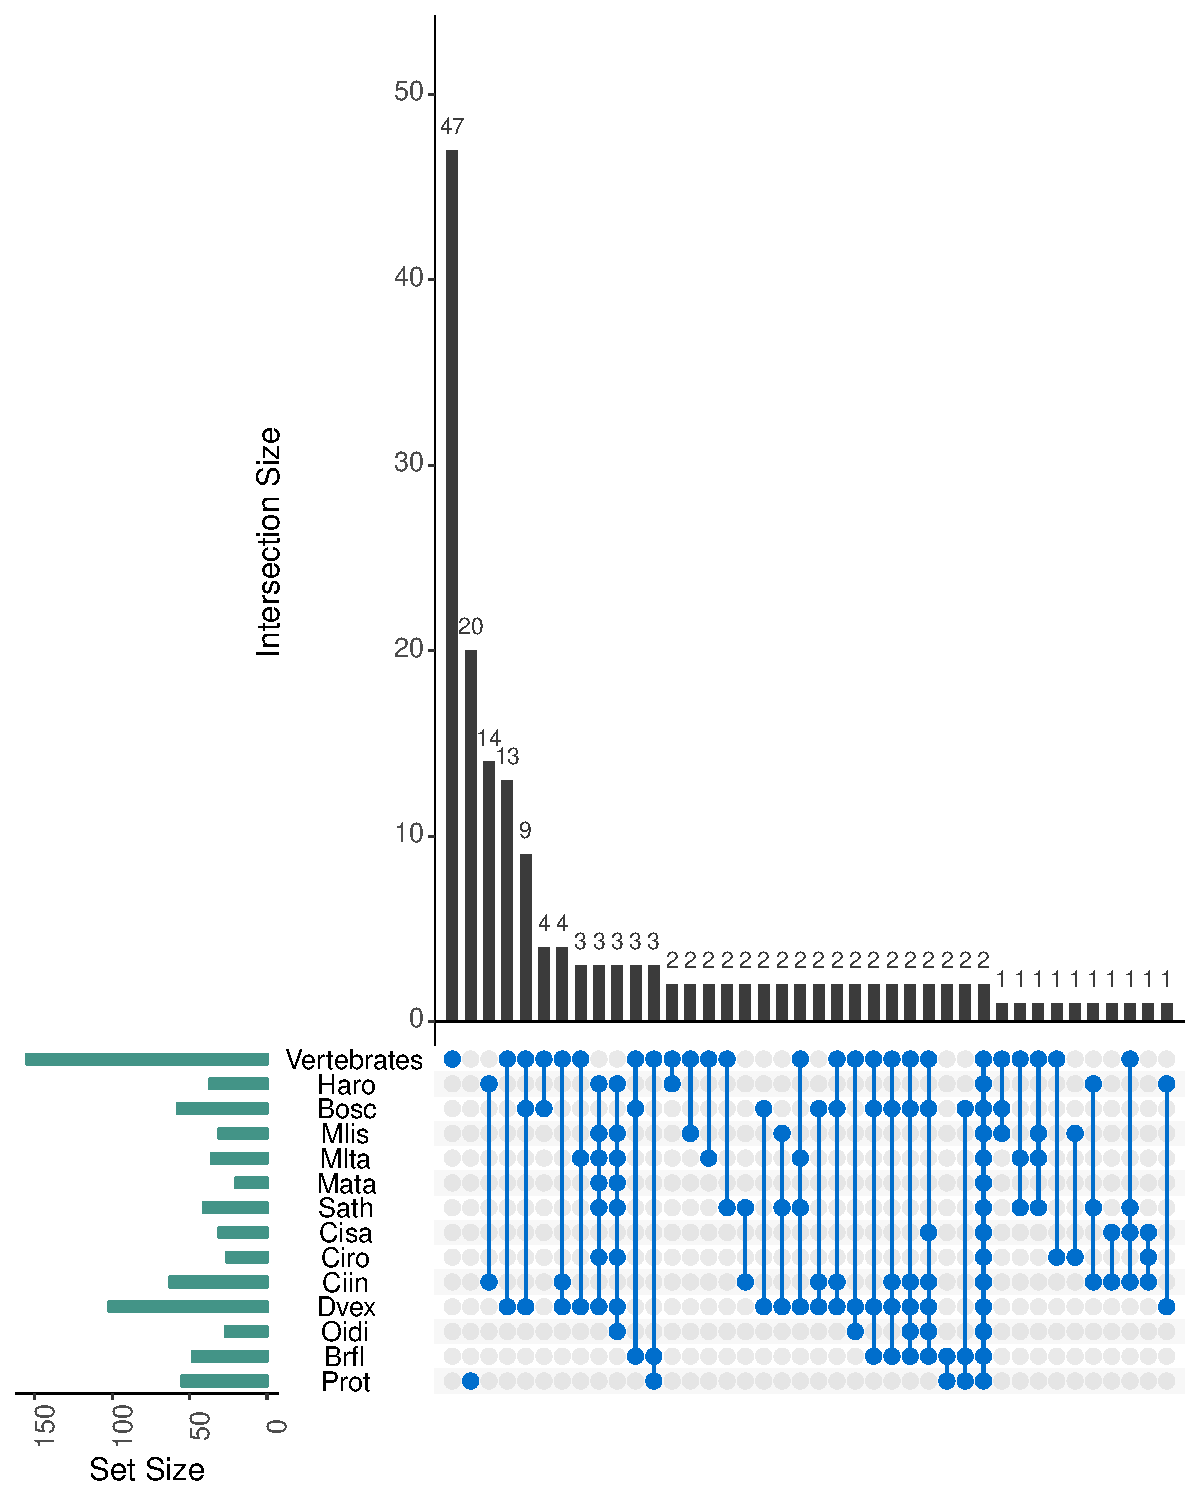
\includegraphics[scale=0.5]{./Images/vennmiRNAs.pdf}
\caption{Comparsion between miRNAs families along Bilaterian species. Same 
labels from Figure \ref{fig:matrimirnas} were used. In this case 
\textsl{vertebrates} group the following species: \textbf{Pema}: \textit{P. 
marinus}, \textbf{Dare}: \textit{D. rerio}, \textbf{Lach}: \textit{L. 
chalumnae}, 
\textbf{Xetr}: \textit{X. tropicalis} and \textbf{Anca}: \textit{A. 
carolinensis}}.
\label{fig:venn}
\end{figure}


\newpage

\bibliographystyle{plain}
\bibliography{tuni.bib}

\end{document}


%%% Local Variables:
%%% mode: latex
%%% TeX-PDF-mode: t
%%% End:
